\section{Approach}
\label{sec:approach}

\begin{figure*}[t]
\centering
\includegraphics[scale=0.66,clip]{figs/approach1.eps}\vspace*{-1ex}
\caption{A high-level overview of our approach} \label{fig:overview}
\end{figure*}

Figure~\ref{fig:overview} shows the high-level overview of our approach. Our approach
includes three major phases: \emph{capture}, \emph{minimize}, and \emph{explore}. In the
capture phase, our approach records dynamic traces from program executions.
Our approach next transforms these dynamic traces into
PUTs and seed tests. Among recorded traces, we identify that there 
many duplicate traces since the same sequence of method calls can 
get invoked multiple times during program executions. Consequently,
the generated PUTs and seed tests also include duplicates.
In the minimize phase, we use a combination of static and dynamic
analyses to filter out duplicate PUTs and seed tests, respectively.
In the explore phase, we use Pex to explore
PUTs to generate regression tests that achieve a high coverage
of the code under test. We next explain each phase in detail.

%------------------------------------------------------------------------
\subsection{Capture Phase}
\label{sec:capture}

In the capture phase, our approach records dynamic traces from program executions. The capture
phase uses a profiler that records method calls invoked by the application
during execution. The capture phase records both the method calls invoked and the concrete
values passed as arguments to those method calls. Figure~\ref{fig:dynamictrace} shows
an example dynamic trace recorded by the capture phase. Statement 2
shows the concrete value ``\CodeIn{<\%\@ Page..$\backslash$u000a}'' passed as an argument
for the \CodeIn{Match} method. Our recorded traces are complete and do not 
require any other primitive values or non-primitive objects. Our recorded traces
include two kinds of methods: state-modifying and observer methods. A method
is referred to as a state-modifying method if the method affects (i.e., writes)
at least one field of its declaring class. A method is referred to as an observer
method if the method does not affect any fields of its declaring class and
also returns a non-void type.

\begin{figure}[t]
\begin{CodeOut}
01: TagRegex tagex = new TagRegex();\\
02: Match mc = ((Regex)tagex).Match("<\%\@ Page..$\backslash$u000a",108);\\
03: Capture cap = (Capture) mc;\\
04: int indexval = cap.Index;\\
\end{CodeOut}\vspace*{-3ex}
\Caption{\label{fig:dynamictrace} An example dynamic trace recorded by 
the capture phase.}\vspace*{-1ex}
\end{figure}

Our approach next generates PUTs and seed tests from recorded traces. 
To generate PUTs, our approach identifies all constant values
and promotes those constant values as parameters. Furthermore, our approach identifies
return values of observer methods in the PUT and
promotes those return values as \CodeIn{OUT} parameters for the PUT. 
In C\#, these \CodeIn{OUT} parameters represent the return values of a method.
Our approach next generates seed tests that includes all concrete values
from the dynamic traces. Figure~\ref{fig:putut} shows a PUT and a seed test
generated from the dynamic trace shown in Figure~\ref{fig:dynamictrace}.

\begin{figure}[t]
\begin{CodeOut}
\textbf{PUT:}\\
00: public static void $F_1$(string $VAL_1$, int $VAL_2$, out int $OUT_1$)\\
01: \hspace*{0.2in}TagRegex tagex = new TagRegex();\\
02: \hspace*{0.2in}Match mc = ((Regex)tagex).Match($VAL_1$, $VAL_2$);\\
03: \hspace*{0.2in}Capture cap = (Capture) mc;\\
04: \hspace*{0.2in}$OUT_1$ = cap.Index;\\
05: \}\\

\textbf{Seed Test:}\\
06: public static void $T_1$() \{\\
07: \hspace*{0.2in}int index;\\
08: \hspace*{0.2in}$F_1$("<\%@ Page..$\backslash$u000a", 108, out index);\\
09: \}\\
\end{CodeOut}\vspace*{-3ex}
\Caption{\label{fig:putut} A PUT and a seed test generated
from the dynamic trace in Figure~\ref{fig:dynamictrace}.}\vspace*{-3ex}
\end{figure}

The generated PUT includes two parameters and one \CodeIn{OUT} parameter.
The \CodeIn{OUT} parameter is the return value of the observer
method \CodeIn{Capture.Index}. These \CodeIn{OUT} parameters are later
used to generate test assertions in regression tests (Section~\ref{sec:explore}). 
The figure also shows a seed test generated from the dynamic trace. 
The seed test includes concrete values of the dynamic trace and invokes the generated PUT with those concrete values.

%------------------------------------------------------------------------
\subsection{Minimize Phase}
\label{sec:minimize}

Our approach records dynamic traces during actual program executions. As the same
sequence of method calls can be invoked multiple times during program executions,
we identify that there are many duplicates among recorded dynamic traces.
Consequently, there are many duplicates among generated PUTs and seed tests. 
In the minimize phase, our approach filters out duplicate PUTs and seed tests.
The primary reason for filtering out duplicates is that exploration of duplicate
PUTs is redundant and can also lead to scalability issues while generating regression tests.

We first present our criteria for a duplicate PUT and a seed test and next explain
how we filter out such duplicate PUTs and seed tests.

\textbf{Duplicate PUT:} We consider a PUT, say $P_1$, as a duplicate
of another PUT, say $P_2$, if both $P_1$ and $P_2$ have the same sequence of method calls. 

\textbf{Duplicate Seed Test:} We consider a seed test, say $S_1$, as a duplicate of 
another seed test, say $S_2$, if both $S_1$ and $S_2$ exercise the same execution path.

\begin{figure}[t]
\begin{CodeOut}
00: void PUT1(int arg1, int arg2, int arg3) \{\\
01: \hspace*{0.2in}if (arg1 > 0)\\
02: \hspace*{0.4in}Console.WriteLine("arg1 > 0"); \\
03: \hspace*{0.2in}else\\
04: \hspace*{0.4in}Console.WriteLine("arg1 <= 0"); \\
05: \hspace*{0.2in}if (arg2 > 0)\\
06: \hspace*{0.4in}Console.WriteLine("arg2 > 0"); \\
07: \hspace*{0.2in}else\\
08: \hspace*{0.4in}Console.WriteLine("arg2 <= 0"); \\
09: \hspace*{0.2in}for (int c = 1; c <= arg3; c++)  \{ \\
10: \hspace*{0.4in}Console.WriteLine("loop") \\
11: \hspace*{0.2in}\}\\
12: \}\\
\\
13: public void SeedTest1() \{\\
14: \hspace*{0.2in}PUT1(1, 1, 1);\\
15: \}\\
\\
16: void PUT2(int arg1, int arg2, int arg3) \{\\
17: \hspace*{0.2in}if (arg1 > 0)\\
18: \hspace*{0.4in}Console.WriteLine("arg1 > 0"); \\
19: \hspace*{0.2in}else\\
20: \hspace*{0.4in}Console.WriteLine("arg1 <= 0"); \\
21: \hspace*{0.2in}if (arg2 > 0)\\
22: \hspace*{0.4in}Console.WriteLine("arg2 > 0");  \\
23: \hspace*{0.2in}else\\
24: \hspace*{0.4in}Console.WriteLine("arg2 <= 0"); \\
25: \hspace*{0.2in}for (int c = 2; c <= arg3; c++)  \{ \\
26: \hspace*{0.4in}Console.WriteLine("loop") \\
27: \hspace*{0.2in}\}\\
28: \}\\
\\
29: public void SeedTest2() \{\\
30: \hspace*{0.2in}PUT2(1, 10, 1);\\
31: \}\\
\\
32: public void SeedTest3() \{\\
33: \hspace*{0.2in}PUT1(5, 8, 2);\\
34: \}\\
\end{CodeOut}\vspace*{-2ex}
\caption{\label{fig:samplePutAndUT}Two PUTs and associated seed tests generated by the capture phase.}\vspace*{-2ex}
\end{figure}

We use PUTs and seed tests shown in Figure~\ref{fig:samplePutAndUT} as 
illustrative examples. The figure shows two PUTs
and three seed tests. Our approach uses static analysis to identify duplicate
PUTs. For example, our approach compares the method bodies of \CodeIn{PUT1} and
\CodeIn{PUT2} at the level of Microsoft Intermediate 
Language\footnote{\url{http://msdn.microsoft.com/en-us/library/c5tkafs1(VS.71).aspx}}
instructions. Our approach ignores any primitive values related to local
variables in the PUTs while comparing instructions. 
In this example, our approach considers \CodeIn{PUT2} as a duplicate of \CodeIn{PUT1},
although the local variable \CodeIn{c} in Statement 9 of \CodeIn{PUT1} is assigned a different value
in \CodeIn{PUT2}. As \CodeIn{PUT2} is a duplicate of \CodeIn{PUT1}, our approach automatically replaces
the \CodeIn{PUT2} method call in \CodeIn{SeedTest2} with \CodeIn{PUT1}.

After filtering out duplicate PUTs, our approach uses dynamic analysis for filtering 
out duplicate seed tests. To identify duplicate seed tests,
our approach executes each seed test and monitors its execution path 
in the code under test. For example, \CodeIn{SeedTest1} follows the 
path ``2 $\rightarrow$ 6 $\rightarrow$ 10'' in \CodeIn{PUT1}. Our approach considers 
\CodeIn{SeedTest2} as a duplicate of \CodeIn{SeedTest1}, as \CodeIn{SeedTest2}
also follows the same path ``2 $\rightarrow$ 6 $\rightarrow$ 10'' in \CodeIn{PUT1}. 
Consider another unit test \CodeIn{SeedTest3} shown in Figure~\ref{fig:samplePutAndUT}.
Our approach does not consider \CodeIn{SeedTest3} as a duplicate of \CodeIn{SeedTest1}
as \CodeIn{SeedTest3} follows the path ``2 $\rightarrow$ 6 $\rightarrow$ 10 $\rightarrow$ 10'',
since \CodeIn{SeedTest3} iterates the loop in Statement 9 two times.

%------------------------------------------------------------------------
\subsection{Explore Phase}
\label{sec:explore}

In the explore phase, our approach uses Pex to generate regression tests from PUTs. Although
seed tests generated in the capture phase can be used as regression tests, those
seed tests exercise only the happy paths such as paths that do not include 
error-handling code in the code under test. Therefore, these seed tests do not
achieve a high coverage of the code under test. 

To address this issue, we use Pex to explore generated PUTs. Inspired by Patrice et al.~\cite{patrice08:whitebox},
we use seed tests to assist Pex during exploration of PUTs. Using seed tests increases
the effectiveness of Pex or any other dynamic-symbolic-execution-based approach in two major ways. First,
seed tests cover several paths in the code under test and Pex can start exploration
from these covered paths rather than starting exploration from the beginning. This 
would reduce the amount of time required in generating tests from PUTs. Second,
seed tests can help cover certain paths that are hard to be covered without using
those tests. For example, it is quite challenging for Pex or any other 
dynamic-symbolic-execution-based approach to generate concrete values for variables
that require complex values such as IP addresses, URLs, doubles. In such scenarios,
seed tests can help by providing desired concrete values to cover those paths.

Pex generated $86$ regression tests for the PUT shown in Figure~\ref{fig:putut}. 
Figure~\ref{fig:generatedtests} shows three sample regression tests generated by Pex.
In regression tests 1 and 2, Pex automatically annotated the unit tests with the expected exceptions
\CodeIn{ArgumentNullException} and \CodeIn{ArgumentOutOfRangeException}, respectively.
Since the PUT (Figure~\ref{fig:putut}) includes an \CodeIn{OUT} parameter, Pex 
generated assertions in regression tests based on actual values captured while 
generating the test. These expected exceptions or assertions serve as test oracles
in regression tests.

\begin{figure}[t]
\begin{CodeOut}
\textbf{Regression Test 1:}\\
00: [PexRaisedException(typeof(ArgumentNullException))]\\
01: public static void $F_{102}$() \{\\
02: \hspace*{0.2in}int i = default(int); \\
03: \hspace*{0.2in}$F_1$ ((string)null, 0, out i);\\
04: \}\\
\\
\textbf{Regression Test 2:}\\
00: [PexRaisedException(typeof(ArgumentOutOfRangeException))]\\
01: public static void $F_{110}$() \{\\
02: \hspace*{0.2in}int i = default(int);\\
03: \hspace*{0.2in}$F_1$("", 1, out i);\\
04: \}\\
\\
\textbf{Regression Test 3:}\\
00: public static void $F_{103}$() \{\\
01: \hspace*{0.2in}int i = default(int);\\
02: \hspace*{0.2in}$F_1$ ("$\backslash$0$\backslash$0$\backslash$0$\backslash$0$\backslash$0$\backslash$0$\backslash$0<$\backslash$u013b$\backslash$0", 7, out i); \\
03: \hspace*{0.2in}PexAssert.AreEqual<int>(0, i);\\
04: \}\\
\\
\end{CodeOut}\vspace*{-5ex}
\Caption{\label{fig:generatedtests} Regression tests generated by Pex by exploring 
the PUT shown in Figure~\ref{fig:putut}.}\vspace*{-5ex}
\end{figure}

Although Pex is effective in exploring PUTs and generating unit tests,
we identify that Pex or any other dynamic-symbolic-execution-based approaches
can lead to scalability issues when handling large number 
of PUTs. To address this issue, our approach uses a distributed 
setup where Pex can explore multiple PUTs in parallel. Our distributed
setup allows to launch multiple Pex processes on several machines.
Once started, our distributed setup is designed to run forever in iterations. 
The primary reason for such a setup is that it is hard to 
decide when to stop exploring a PUT. For example, loops in the
code under test introduce infinite number of possible paths and 
it will take infinite amount of time to generate tests.

To address the preceding issue, we explore PUTs in iterations bounded by
various parameters. For example, consider a timeout parameter that describes
when to stop exploring a PUT. In the first iteration, we set three minutes
for the timeout parameter. This timeout parameter indicates that we terminate
exploration of a PUT after three minutes. In the first iteration, we explore all PUTs with
these bounded parameters. In the second iteration, we double the values
of these parameters. For example, we set six minutes for the timeout parameter
in the second iteration. Doubling the parameters gives more time for
Pex in exploring new paths in the code under test. 
To avoid Pex exploring the same paths that were explored in previous iterations, we 
maintain a pool of all generated tests. We use the tests in the pool generated
by previous iterations as a seed for further iterations.
For example, tests generated in Iteration 1 are used as seed tests in Iteration 2. 
